\chapter{Erstellung der neuen Komponentenbibliothek}
\label{cha:Neue Komponentenbibliothek}

\section{Anforderungen}
Die derzeit eingesetzte Komponentenbibliothek aus dem Repository \textit{portal-global-components} wurde zuerst auf Basis von vue-cli 2 und nach späterer Migration auf vue-cli 3 entwickelt. Es werden bis jetzt keine Dokumentations-Frameworks verwendet und die Dokumentierung der erstellten Bibliothek wird manuell als eigene Vue-App entwickelt.

Aufgrund der bestehenden Komplexität, die unteranderem Resultat der in Kapitel \ref{cha:Herausforderungen im Frontend} aufgelistet Herausforderungen ist, und dem bevorstehenden  UI-Redesigns des gesamten Portals soll eine neue Komponentenbibliothek der Frontend-Infrastruktur hinzugefügt werden. Diese soll zu einer Verbesserung der in Kapitel \ref{cha:Herausforderungen im Frontend} genannten Herausforderungen beitragen und außerdem das Utility-Class Framework Tailwind CSS verwenden und somit im Frontend einführen. Sowohl die bestehende Bibliothek als auch die neue Bibliothek sollen zunächst im Frontend verwendet werden. Ab Release der neuen Bibliothek soll diese jedoch das \textit{portal-global-components} Repository langfristig vollständig ersetzen.

Anforderungen, die sich für die neue Vue-Komponentenbibliothek ergeben sind folglich:
\begin{itemize}
    \item \textbf{Einführung von Tailwind CSS}: Unter Verwendung der Bibliothek wird Tailwind CSS auch in \textit{portal-frontend} eingeführt. Die Bibliothek liefert eine Standard-Tailwind-Konfiguration, die in Portal-Instanzen individuell angepasst werden kann.
    \item \textbf{Isolierte Komponentenentwicklung}: Die Komponenten sollen unabhängig von \textit{portal-frontend} und einer Portal-Koniguration entwickelt werden sowie nutzbar sein (vgl. Abschnitt \ref{sec:portalConfigDep}).
    \item \textbf{Automatisierte Komponentendokumentation}: Die Komponenten sollen nicht mehr vollständig manuell von Entwickelnden dokumentiert werden. Stattdessen soll der Entwickler eine \textit{Single-File-Component} mit mindestens einem Codebeispiel neu einführen können. Anschließend sollen dann beispielsweise Properties und Codebeispiele benutzerfreundlich in einer Vue-Single-Page-Application dargestellt werden \ref{sec:manualDocumentation}).
    \item \textbf{Einfache Komponentenkategorisierung}: Komponenten sollen weiterhin gemäß ihrer Komplexität in entsprechende Ordner gespeichert werden. Die Probleme aus Abschnitt \ref{sec:componentManagement}) sollen dabei weitesgehend gelöst werden.
  \end{itemize}

\section{Frameworkwahl}
Damit die neue Bibliothek möglichst robust ist und die Einführung möglichst einfach umzusetzen ist, soll ein passendes Framework als Projektbasis eingesetzt werden. Zunächst wird ein Vergleich zwischen drei möglichen Frameworks präsentiert um schließlich eine Auswahl treffen zu können.

\subsection{Vergleich}
\label{sec:frameworkComparision}
Nach einer Recherche wurden für dieses Projekt drei Open-Source Frameworks näher betrachtet.

\defcitealias{VueStyleguidist}{\usebibentry{VueStyleguidist}{title}}
\defcitealias{VueDesignSystem}{\usebibentry{VueDesignSystem}{title}}
\defcitealias{Storybook}{\usebibentry{Storybook}{title}}

\begin{enumerate}
    \item \textbf{\citetalias{VueStyleguidist}} (1,8k Follower auf \cite{VueStyleguidistGithub})\newline
    Vue-Styleguidist ist ein Fork des bekannten react-styleguidist (9,2k Follower auf \cite{ReactStyleguidistGithub}). Vue Styleguidist wird offiziell als \emph{``Isolated Vue component development environment with a living style guide.''} \citep{VueStyleguidist} beschrieben. Das Framework kann basierend auf Code-Kommentare einer Komponente eine Dokumentation dieser automatisiert anfertigen. Dokumentationsseiten werden in Markdown verfasst. Außerdem ist dieses Framework offiziell Teil des Vue-Community-Ecosystems\footnote{ \url{https://vue-community.org/guide/ecosystem/documentation.html\#vue-styleguidist } }, was einen langen Support mit regelmäßigen Updates wahrscheinlich macht.
    \item \textbf{\citetalias{VueDesignSystem}} (1,9k Follower auf \cite{VueDesignSystemGithub})\newline
    Das Vue Design System wurde von Viljami Salminen, einem Design System Architekten aus Finland, erstellt und wurde bereits in der Vergangenheit von der AVACO GmbH für eine neue Bibliothek in Betracht gezogen. Das Projekt basiert auf Vue.js und Vue-Stylguidist. Dabei unterscheidet es sich besonders darin eigene Design-System-Praktiken und Strukturen dem Anwendenden anzubieten. Eine Praktik stellt dabei eine abstraktere Atomic Design Alternative dar. Diese ist besonders im Hinblick auf Komponentenmanagement Herausforderung aus Abschnitt \ref{sec:componentManagement} interessant.

    Die Terminologie des abgewandelten Atomic Design Ansatzes werden wir folgt definiert \citep{VueDesignSystemTerminology}:
    \begin{itemize}
        \item \textbf{Design Tokens}: Werden in einer .yml Datei definiert und sind im gesamten Design System als SASS-Variablen nutzbar.
        \item \textbf{Elements}: Komponenten, die nicht weiter heruntergebrochen werden können. Beispielsweise Buttons.
        \item \textbf{Patterns}: Komponenten, die aus anderen \textit{Elements} und \textit{Tokens} bestehen.
        \item \textbf{Templates}: Komponenten, die aus \textit{Elements}, \textit{Patterns} und \textit{Tokens} bestehen
    \end{itemize}

    Der letzte Release erfolgte im Jahr 2018 weshalb man derzeit nicht beurteilen kann inwieweit das Projekt noch gepflegt werden wird. Vue-Styleguidst, das Basisframework, erhält jedoch weiterhin Updates.
    \item \textbf{\citetalias{Storybook}} (53,7k Follower auf \cite{StorybookGithub})\newline
    Storybook ist ein populäres aus der React-Community entstandendes Framework. Die offizielle Beschreibung lautet wie folgt:

    \begin{quotation}
        \emph{``Storybook is an open source tool for developing UI components in isolation for React, Vue, Angular, and more. It makes building stunning UIs organized and efficient.''} \citep{Storybook}
    \end{quotation}

    Obwohl das Framework ursprünglich für React entwickelt wurde unterstützt es mittlerweile in weiten Umfängen viele weitere Frameworks. Komponenten werden dabei in \textit{Stories} dokumentiert, welche in einer eigenen JavaScript-Datei gespeichert werden. Eine Vue-Story wird dann als Stringified Single Page Component verfasst. Dieser Prozess ist nicht vollkommen automatisiert, da zu einer neuen Komponente zunächst eine Story verfasst werden muss. Die Story kann in Form eines Beispielcodes verfasst werden. Jede Komponente, die in eine Story als Modul hineingeladen wird, wird dann automatisiert analysiert und Properties, Slots, etc. benutzerfreundlich dargestellt.

    Insgesamt ist Storybook durch seine Schnittstellen und Pluginsystem sehr mächtig. Dies geschieht jedoch auf Kosten der initialen Aufsetzung.

    Zwei weitere interessante Eigenschaften sind zum einen die Svelte\footnote{ Mehr zu Svelte: \url{https://svelte.dev/} } Unterstützung und zum anderen die Figma-Einbindungsmöglichkeit, da die AVACO GmbH diese beiden Werkzeuge in Zukunft zusätzlich einführen könnte.
\end{enumerate}

\subsection{Auswahl Storybook}
\cite{WorkshopStorefront} definiert in seinem Artikel die Bezeichnungen \textit{Workshop} und \textit{Storefront} in Bezug auf Design-Systeme. Demnach sind \textit{Workshops} Entwicklungsumgebungen für das effektive Erstellen neuer UI-Komponenten im Team. Der \textit{Workshop} bietet alle Werkzeuge und Strukturen für diese Arbeit.

Die \textit{Storefront} präsentiert hingegen das fertige Design-System mit allen weiteren Ressourcen. Ähnlich zu einem Styleguide sollen in der \textit{Storefront} Informationen erscheinen, die für Entwickler und Benutzer aus anderen Disziplinen hilfreich sind.

Laut \cite{StorybookVSStyleguidist} dem Initiator von Storybook haben Styleguidist und Storybook viele Gemeinsamkeiten und bedienen beide jeweils Anforderungen an Workshop und Storefront. Jedoch klassifiziert er letztendlich Styleguidist als Storefront und Storybook als Workshop. Auch \cite{FrostCite} bezeichnet Storbook wie folgt:
\begin{quotation}
    \emph{``Storybook is a powerful frontend workshop environment tool that allows teams to design, build, and organize UI components (and even full screens!) without getting tripped up over business logic and plumbing.''}
\end{quotation}
Da es in diesem Projekt besonders darum geht eine robuste Komponentenbibliothek für Frontend-Entwickler zu erstellen, welche die Entwickler in ihren Entwicklungen unterstützt und die Entwickler nur einfache Storefront-Eigenschaften benötigen wird das Projekt mit Storybook entwickelt. Jedoch sollen die von \citep{VueDesignSystemTerminology} definierten Terminologien und Prinzipien bei der Umsetzung auf das Tailwind-Ecosystem projiziert werden. Sofern in Zukunft die Bibliothek um ein vollständiges Design System erweitert werden sollte, sollte ein zusätzliches Werkzeug zur Dokumentierung und Darstellung des Systems gesucht werden.

\section{Entwicklung}
\subsection{Repositoryverwendung}
Die Komponenten Bibliothek wird in einem eigenen Repository unter dem Namen \textit{portal-storybook} erstellt und kann anschließend als \textit{Node-Module} in anderen Projekten als Vue-Plugin installiert werden. Dabei soll die Bibliothek drei unterschiedliche Komponenten-Registrierungen ermöglichen.

\begin{enumerate}
    \item \textbf{Installation aller Komponenten im globalen Vue Namespace}: Komponenten müssen zur Verwendung nicht mehr in andere Dokumente importiert werden, sondern können direkt im Markup unter ihrem Komponenten-Namen genutzt werden.
\begin{lstlisting}[language=JavaScript , caption={Globale Installierung},label={lst:GlobalInstall}]
// bspw. main.js in einem vue-cli-3 Projekt
// ...
import * as storybook from 'portal-storybook'
// ...
Vue.use(storybook, {useAllComponents: true})
\end{lstlisting}
    \item \textbf{Installation einzelner Komponenten als Modul durch \textit{Named Exports} aus der Dependency heraus}: Komponenten werden nicht im globalen Namespace installiert sondern werden erst spezifisch in den Dokumenten wo sie genutzt werden durch \textit{Named Imports} als Komponente installiert. In der \textit{main.js} aus \ref{lst:GlobalInstall} würde jedoch weiterhin \textit{Vue.use(storybook, {})} ohne dem useAllComponents-Key aufgerufen werden um andere notwendige Abhängigkeiten zu registrieren. 
\begin{lstlisting}[language=JavaScript , caption={Named Exports/Imports in einer SFC},label={lst:NamedExports}]
// bspw. eine Datei mit dem Namen Dashboard.vue im
// ...
<script>
import { MyComponent1, MyComponent2 } from 'portal-storybook'

export default {
    components: { MyComponent1, MyComponent2 } 
}
</script>
\end{lstlisting}
    \item \textbf{Installation einzelner Komponenten als Modul durch import der SFC Vue-Dateien aus dem Dependecy-Verzeichnis}: Sofern Treeshaking in einem Projekt nicht unterstützt wird und eine globale Installation nicht erfolgen soll können Komponenten außerdem auch durch einzelne Imports installiert werden.
\begin{lstlisting}[language=JavaScript , caption={Default Exports/Imports in einer SFC},label={lst:NamedExports}]
// bspw. eine Datei mit dem Namen Dashboard.vue im
// ...
<script>
import MyComponent1 from 'portal-storybook/src/elements/MyComponent1'
import MyComponent1 from 'portal-storybook/src/elements/MyComponent2'

export default {
    components: { MyComponent1, MyComponent2 } 
}
</script>
\end{lstlisting}
\end{enumerate}
\subsection{Repositoryaufbau}
\label{sec:repoaufbau}
Wie bereits im Vorwort erwähnt wird in dieser Arbeit nicht das Orginal-Repository \textit{portal-storybook} aus dem Firmeneigentum der AVACO GmbH referenziert sondern eine andere Komponentenbiliothek (\textit{tailwindstories}) die auf den selben Konzepten und Lösungen aufbaut, nicht die Firmenkomponenten enthält und neu aufgetauchte Probleme aus \textit{portal-storybook} (vgl. \ref{sec:newChallenges}) bereits mitbehandelt.

Die Abbildung \ref{fig:repoStorybook} am Ende dieses Kapitels zeigt einen Screenshot des \textit{tailwindstories}-Repository und stellt den Verzeichnisaufbau nach der Einführung von storybook in ein neues \textit{vue-cli-3} Vue-Projekt (v.2.) da.

Neben diversen Konfigurationsdateien gibt es die folgenden hervorzuhebenden Verzeichnisse und Dateien:
\begin{itemize}
    \item \textbf{.storybook}\newline
    Enthält alle Storybook spezifisch Workbench-Konfigurationen und Funktionen. Diese sind wichtig für die Nutzung der Workbench, werden aber für den Import fertiger Komponente in einem anderen Projekt nicht benötigt.
    \item \textbf{src/main.js}\newline
    Entrypoint-Datei für die Nutzung als Bibliothek mit Setup-Methoden und Bibliothek-Konfigurationen.
    \item \textbf{src/elements}\newline
    Verzeichnis mit Komponenten die als \textit{elements} klassifiziert werden. Komponenten werden als Vue-SFC-Dateien angelegt, in der index.js importiert und dann als Named-Modul in der main.js importiert. Eine README.md erklärt die Klassifizierungsmerkmale laut Salminen:
    \begin{quotation}
        \emph{``Elements utilize decisions made on the token level. A simple example of an element would be a button, a link, or an input. Anything that cannot be broken down further. I use the name ‘element’ since everything in Vue and React world is nowadays ‘a component.’ Using that term for anything else would be confusing.''} \citep{VUEDSElements}
    \end{quotation}
    \item \textbf{src/patterns}\newline
    Verzeichnis mit Komponenten die als \textit{patterns} klassifiziert werden. (wie \textit{src/elements})
    \begin{quotation}
        \emph{``Patterns are UI Patterns that fall on the more complex side of the spectrum. So for example things like a date picker, a data table, or a visualization. Patterns utilize both elements and tokens. 
        If you wonder whether something should be called an element or a pattern, ask yourself this question: “Can this be broken down into smaller pieces?” If the answer is yes, it should most likely be a pattern.''} \citep{VUEDSPatterns}
    \end{quotation}
    \item \textbf{src/templates}\newline
    Verzeichnis mit Komponenten die als \textit{templates} klassifiziert werden. (wie \textit{src/elements})
    \begin{quotation}
        \emph{``Templates exist to document the layout and structure of a section. I am not calling these pages since semantically that would be incorrect. While they can be pages, that’s not their only functionality. Templates consist of the three things mentioned above: tokens, elements, and patterns.''} \citep{VUEDSTemplates}
    \end{quotation}
    \item \textbf{src/plugins}\newline
    Verzeichnis mit Tailwind-Plugins die unter anderem als \textit{Tokens} klassifiziert werden können.
    \begin{quotation}
        \emph{``Design tokens are the visual design atoms of the design system — specifically, they are named entities that store visual design attributes. We use them in place of hard-coded values (such as hex values for color or pixel values for spacing) in order to maintain a scalable and consistent visual system for UI development.''} \citep{DesignTokens}
    \end{quotation}
    Die Tailwind CSS Plugins können Tokens als neue Utility-Klassen einführen.\footnote{Mehr zu Tailwind CSS Plugins: \url{https://tailwindcss.com/docs/plugins}}
\end{itemize}

\begin{figure}[!ht]
	\centering
		%[natürliche Breite in Pixeln, natürliche Höhe in Pixeln, Abhängigkeit von der Textbreite]
		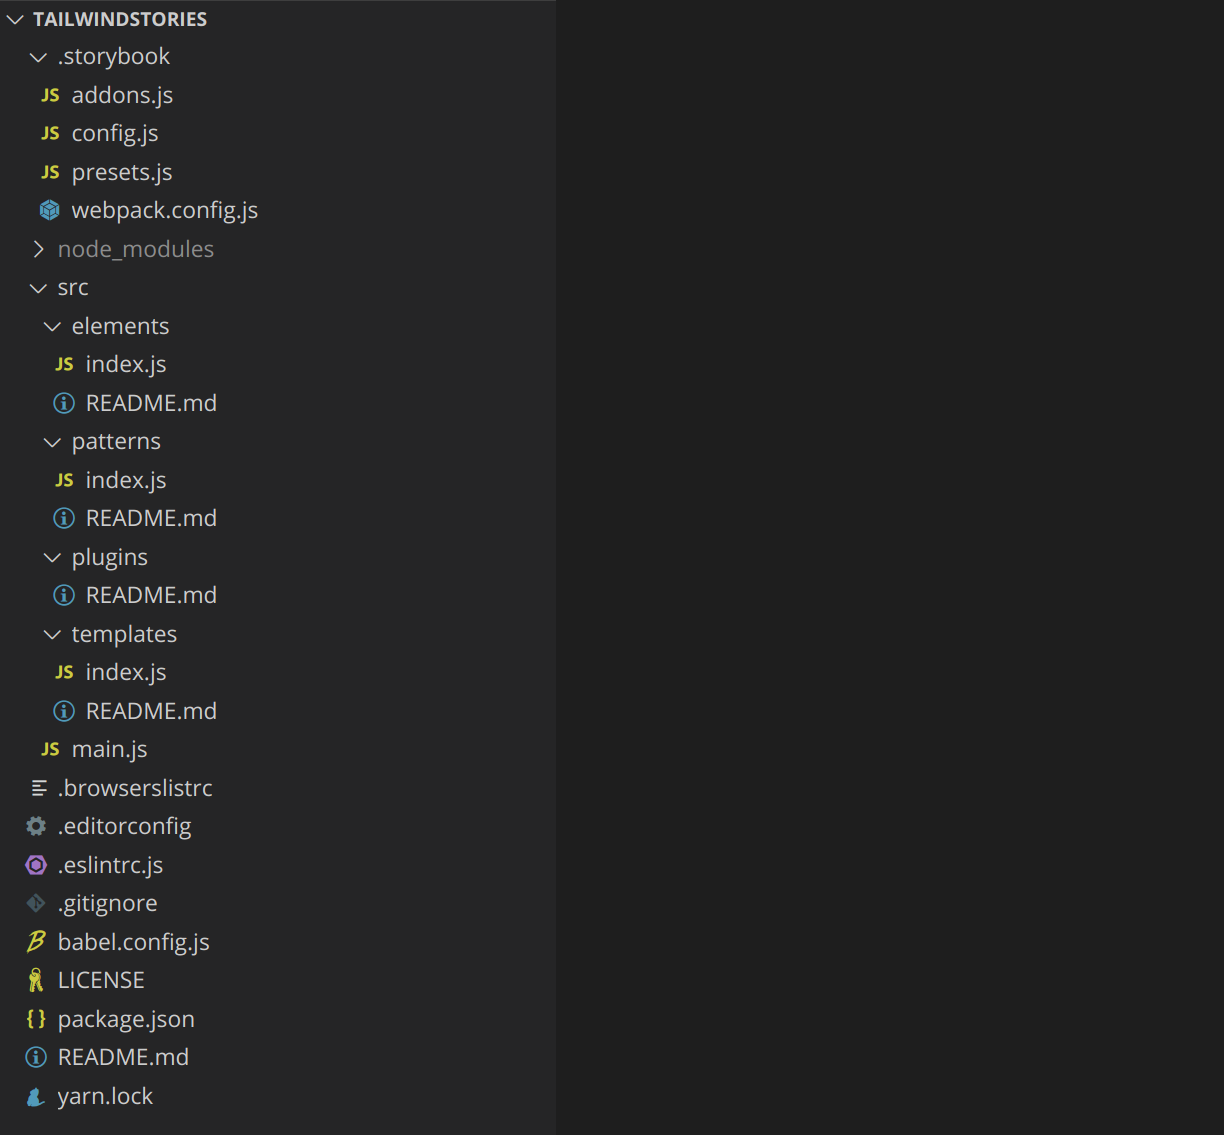
\includegraphics[width=.85\textwidth]{images/004-000-001-repo-storybook.png}
	\caption{Repositoryaufbau mit Storybook}
	\label{fig:repoStorybook}
\end{figure}

\subsection{Storybook Setup}
\label{sec:storybooksetup}
Zu Beginn des Projektes wurde Storybook Version 4 in \textit{portal-storybook} installiert und eingesetzt. Zur automatisierten Dokumentation der erstellten Vue-Komponenten wurde das Addon \textit{storybook-addon-vue-info}\footnote{Repository: \url{https://github.com/pocka/storybook-addon-vue-info}} eingesetzt. Dieses Addon kann die genutzten Komponenten in einer Story analysieren und wichtige Eigenschaften sowie den Quellcode in dem Storybook-GUI nutzerfreundlich darstellen.

Seit der Storybook Version 6 wird das Storybook Addon \textit{@storybook/addon-info} auf welchem das Addon \textit{storybook-addon-vue-info} basiert nicht mehr unterstützt und Storybook bietet nun offiziell das Addon \textit{@storybook/addon-docs} für den Zweck automatisierter Komponenten-Analysen an. Dieses Addon arbeitet derzeit besonders gut mit React Komponenten aber auch Vue Komponenten können analysiert und mit ihren Eigenschaften dargestellt werden. Es gibt die Möglichkeit Property-Werte direkt aus der GUI heraus zu manipulieren. Der einzige Nachteil im Vergleich zu dem nun veralteten (deprecated) \textit{storybook-addon-vue-info} ist, dass Code-Snippets derzeit nicht den eigentlichen Code der dargestellten Komponente enthalten, sondern den Code der Story \citep{GithubIssueStorybook}. In React mit JSX tritt dieses Problem jedoch nicht auf.

Da dies jedoch für eine gute Developer-Expierence behindernd ist, wurde \textit{tailwindstories} zunächst auch nicht auf der Storybook Version 6 aufgebaut sondern auf der Version 5 zusammen mit \textit{storybook-addon-vue-info}. In der Zukunft soll jedoch ein Upgrade auf Version 6 mit \textit{@storybook/addon-docs} ausgeführt werden.

\subsection{Komponentengruppierung}
In Abschnitt \ref{sec:repoaufbau} wurde bereits der generelle Aufbau des Repositorys erläutert jedoch soll im folgenden ein weiteres Prinzip zum Management mit Komponenten präsentiert werden um die globalen Komponentenordner \textit{elements}, \textit{patterns} und \textit{templates} nicht mit kontextgebundenen Komponenten, wie in Codebeispiel \ref{Komponenten Management - Navbar.vue} gezeigt zu füllen.


Generell können sollen Komponenten nach Charakteristiken in Unterordnern eingeordnet werden. So können beispielsweise Formular-Elemente wie Inputs, Textareas, Datum-Selektoren in \textit{elements/form} eingeordnet werden. Jede Vue-Komponenten-Datei soll mit einem Großbuchstaben anfangen, dass beispielsweise in \textit{elements/form} die Dateien \textit{FormInput.vue} und \textit{FormTextarea.vue} befinden. Ein weiteres Merkmal ist der Prefix \textit{Form} in den Dateinamen. Dieser hilft den Entwicklern den Ort der Komponente zu identifizieren. Der Prefix orientiert sich immer an den letzten Ordnername des Dateiweges. Würde man den Ordner \textit{form} in einem weiteren Ordner einnisten so würden sich die Dateinamen nicht ändern. Ein Gruppierungsordner soll immer mit einem Kleinbuchstaben anfangen.

Die Lösung für das Problem mit der Einordnung von kontextgebundenen Komponenten gestaltet sich nun so, dass ein Komponente wie \textit{Navbar.vue} beispielsweise in \textit{patterns/Navbar/Navbar.vue} eingeordnet werden kann. Der Ordner \textit{Navbar} beginnt wie eine Komponete mit einem Großbuchstaben und darf in einem \textit{\_components}-Ordner \textit{elements}, \textit{patterns} und \textit{templates} unkategorisiert enthalten. Diese Komponenten sind jedoch nur im Kontext von \textit{Navbar.vue} zu verwenden, entweder als Kind in einem Slot einer Navbar.vue Instanz oder in der SFC von Navbar.vue. Der Prefix dieser Komponente richtet sich an den Ordnernamen über \textit{\_components}; in diesem Fall \textit{Navbar}. Das folgende Beispiel soll den Aufbau verdeutlichen. 

\lstinputlisting[caption={components/patterns/Navbar/Navbar.vue}, label={KomponentenManagementLoesungNavbar.vue}]{code/004-000_komponentenbib/KomponentenManagement.vue}


